
\hspace{-0.4cm}
\begin{sidewaysfigure}
  \vspace{0.6cm}
  %\hspace{0.5cm}
  \begin{subfigure}[t]{0.32\textwidth}
    \centering
    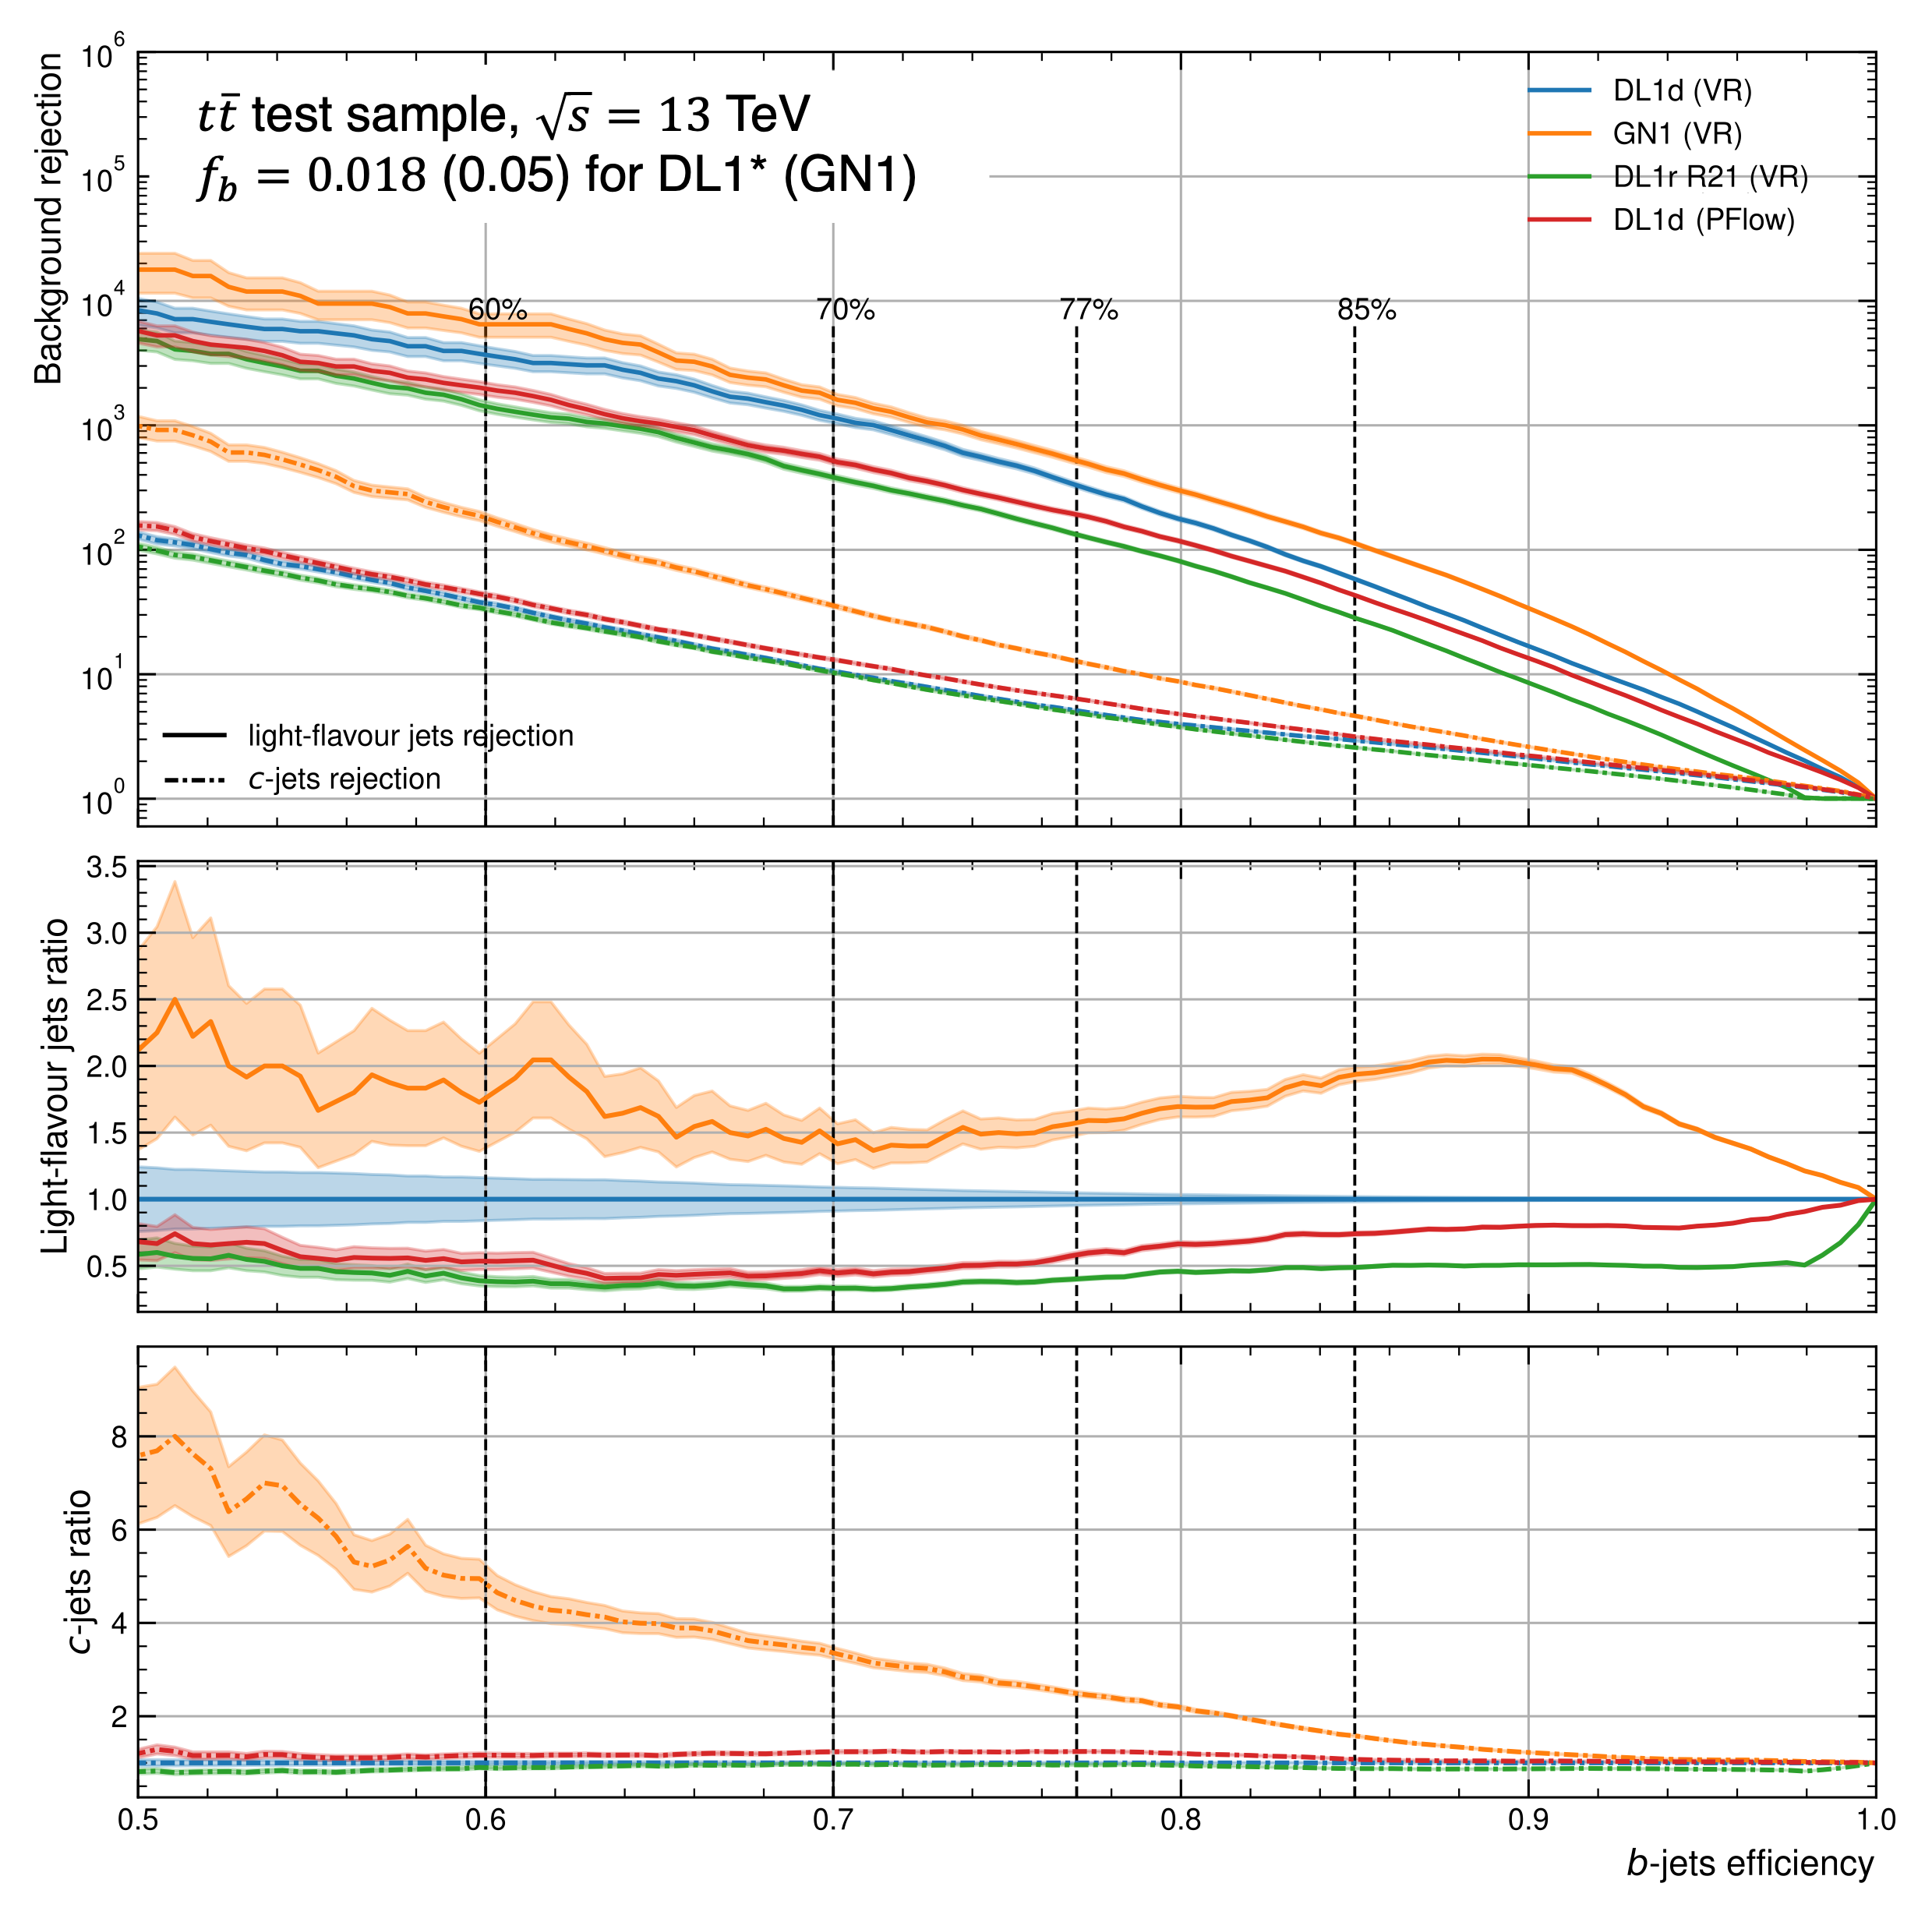
\includegraphics[width=\textwidth]{Images/FTAG/VRDL1d/ROC/ttb.png}
    \caption{$t\bar{t}$ test sample $b$-tagging, $f_c = 0.018$ for DL1d.}
    \label{fig:dl1dVRROCtt}
  \end{subfigure}
  \hfill
  \begin{subfigure}[t]{0.32\textwidth}
    \centering
    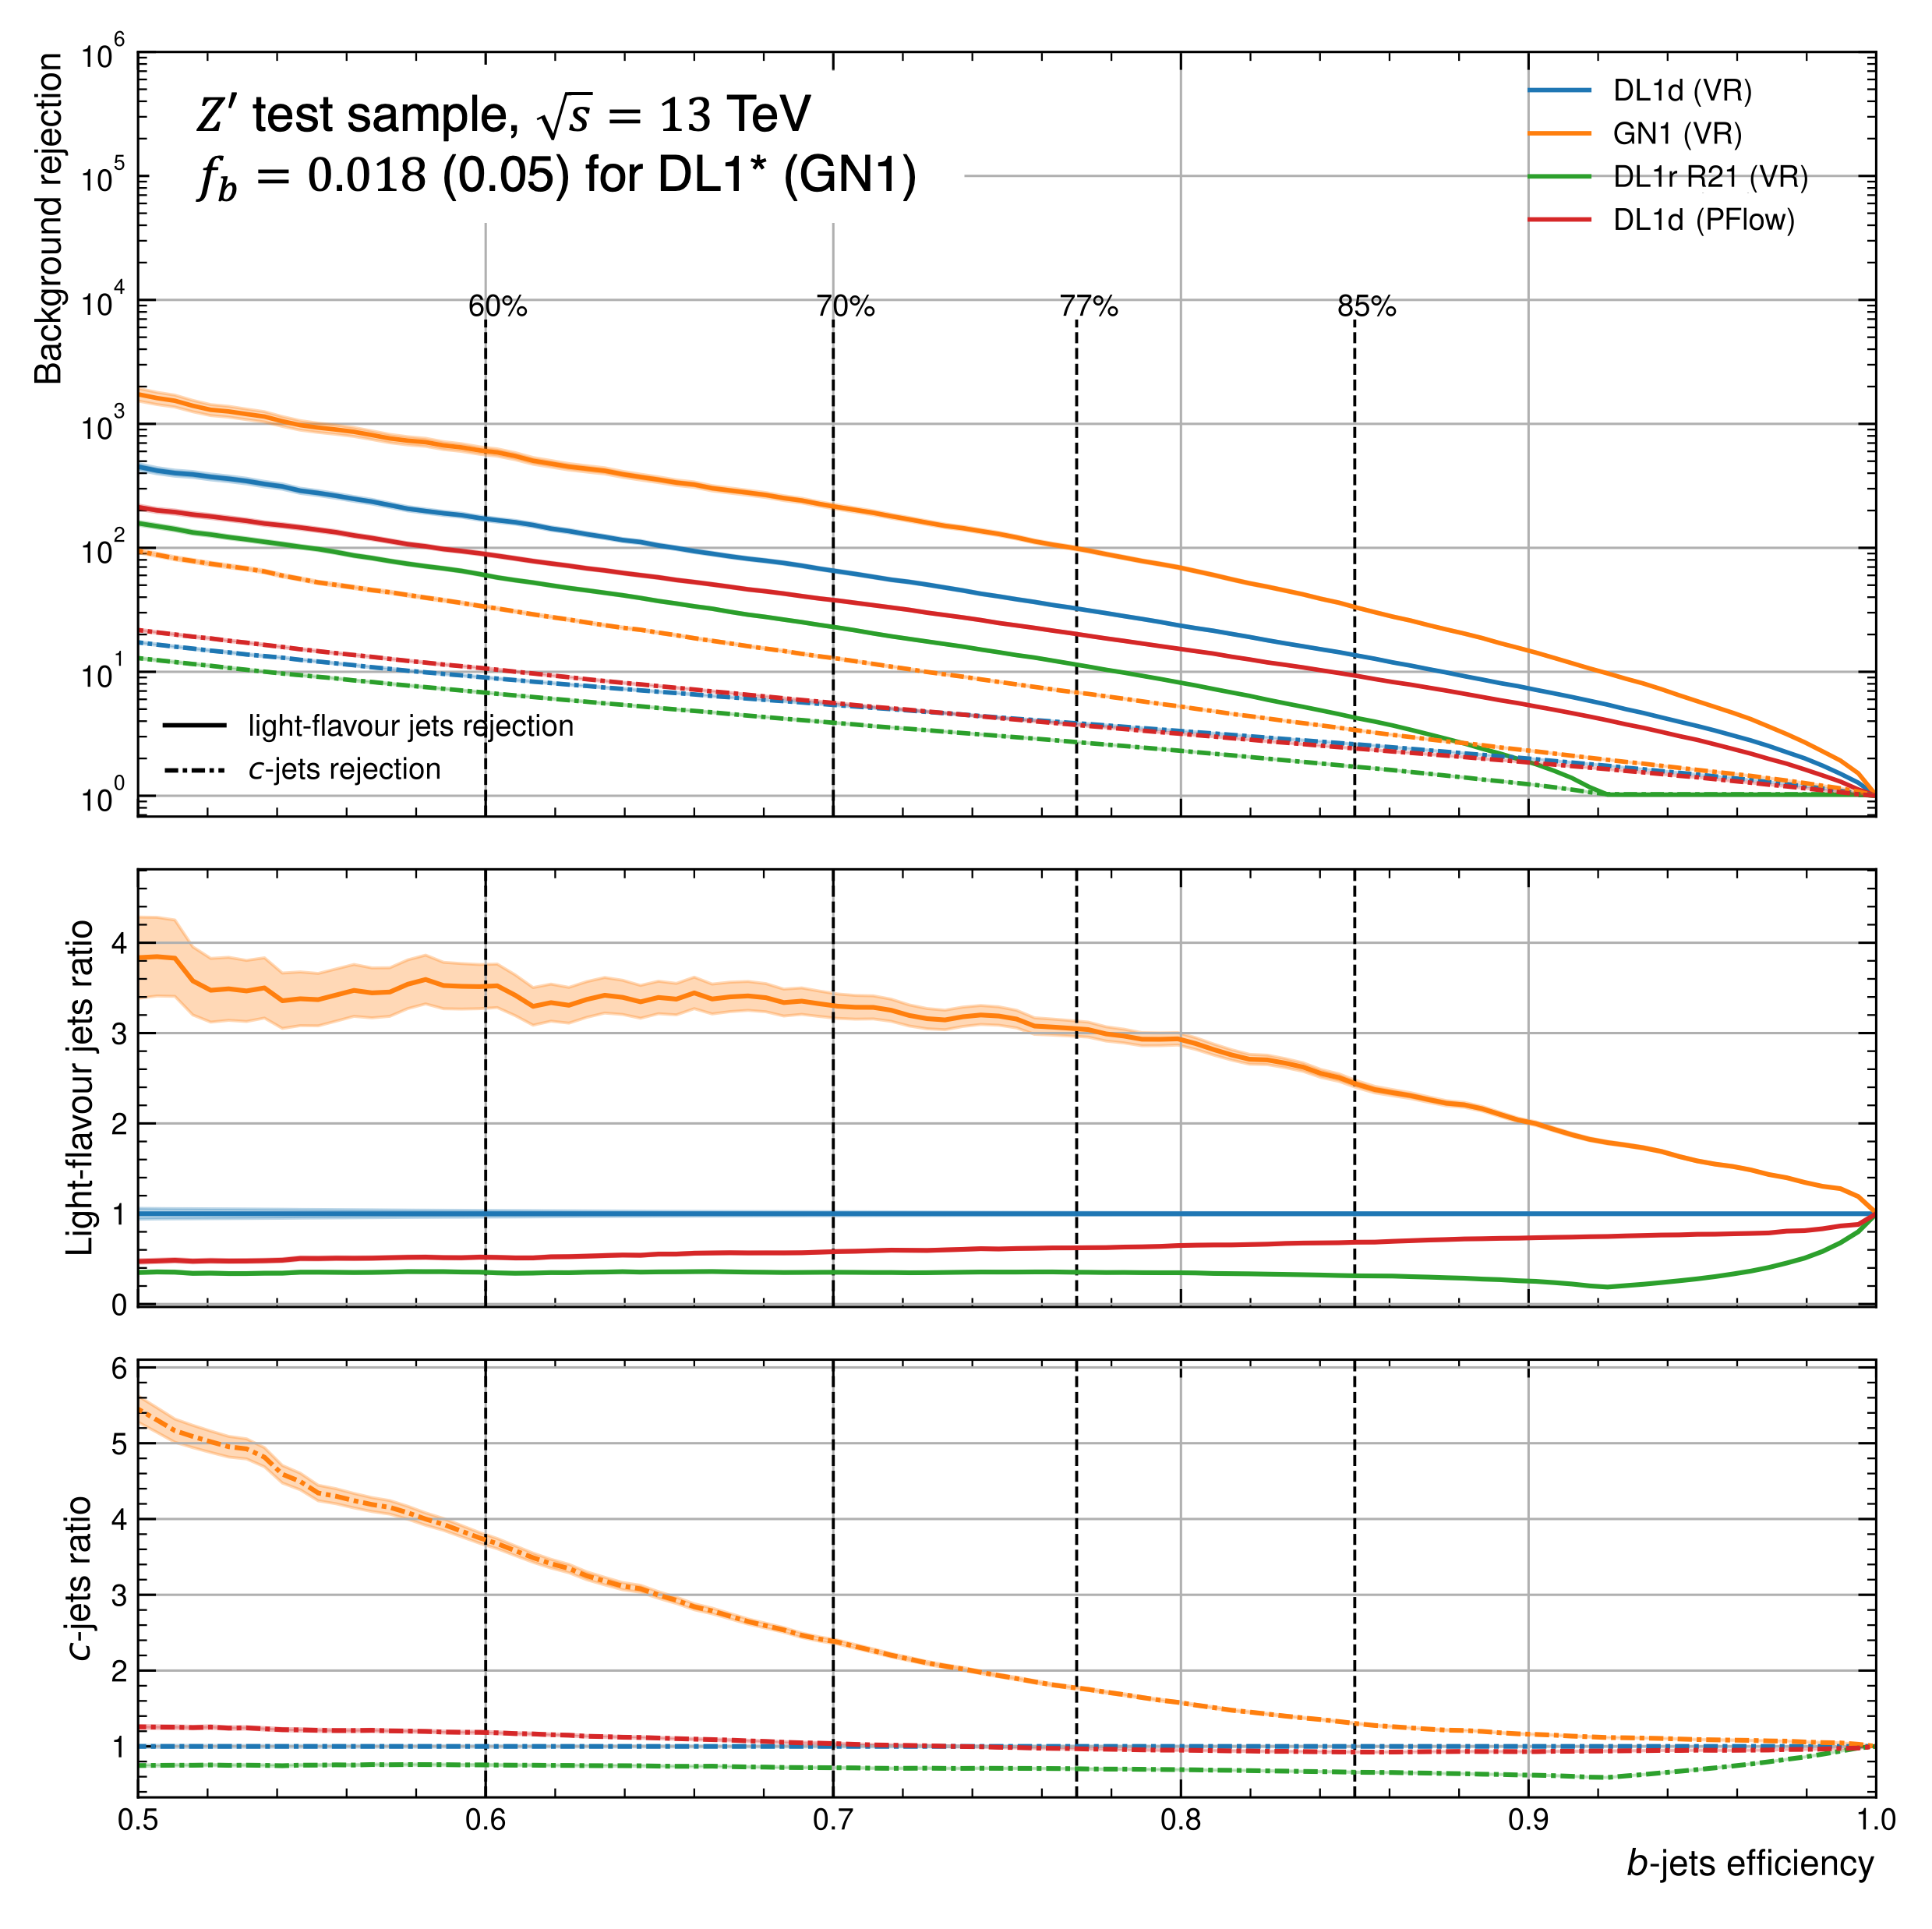
\includegraphics[width=\textwidth]{Images/FTAG/VRDL1d/ROC/zpb.png}
    \caption{$Z'$ test sample $b$-tagging, $f_c = 0.018$ for DL1d.}
    \label{fig:dl1dVRROCzp}
  \end{subfigure}
  \hfill
  \begin{subfigure}[t]{0.32\textwidth}
    \centering
    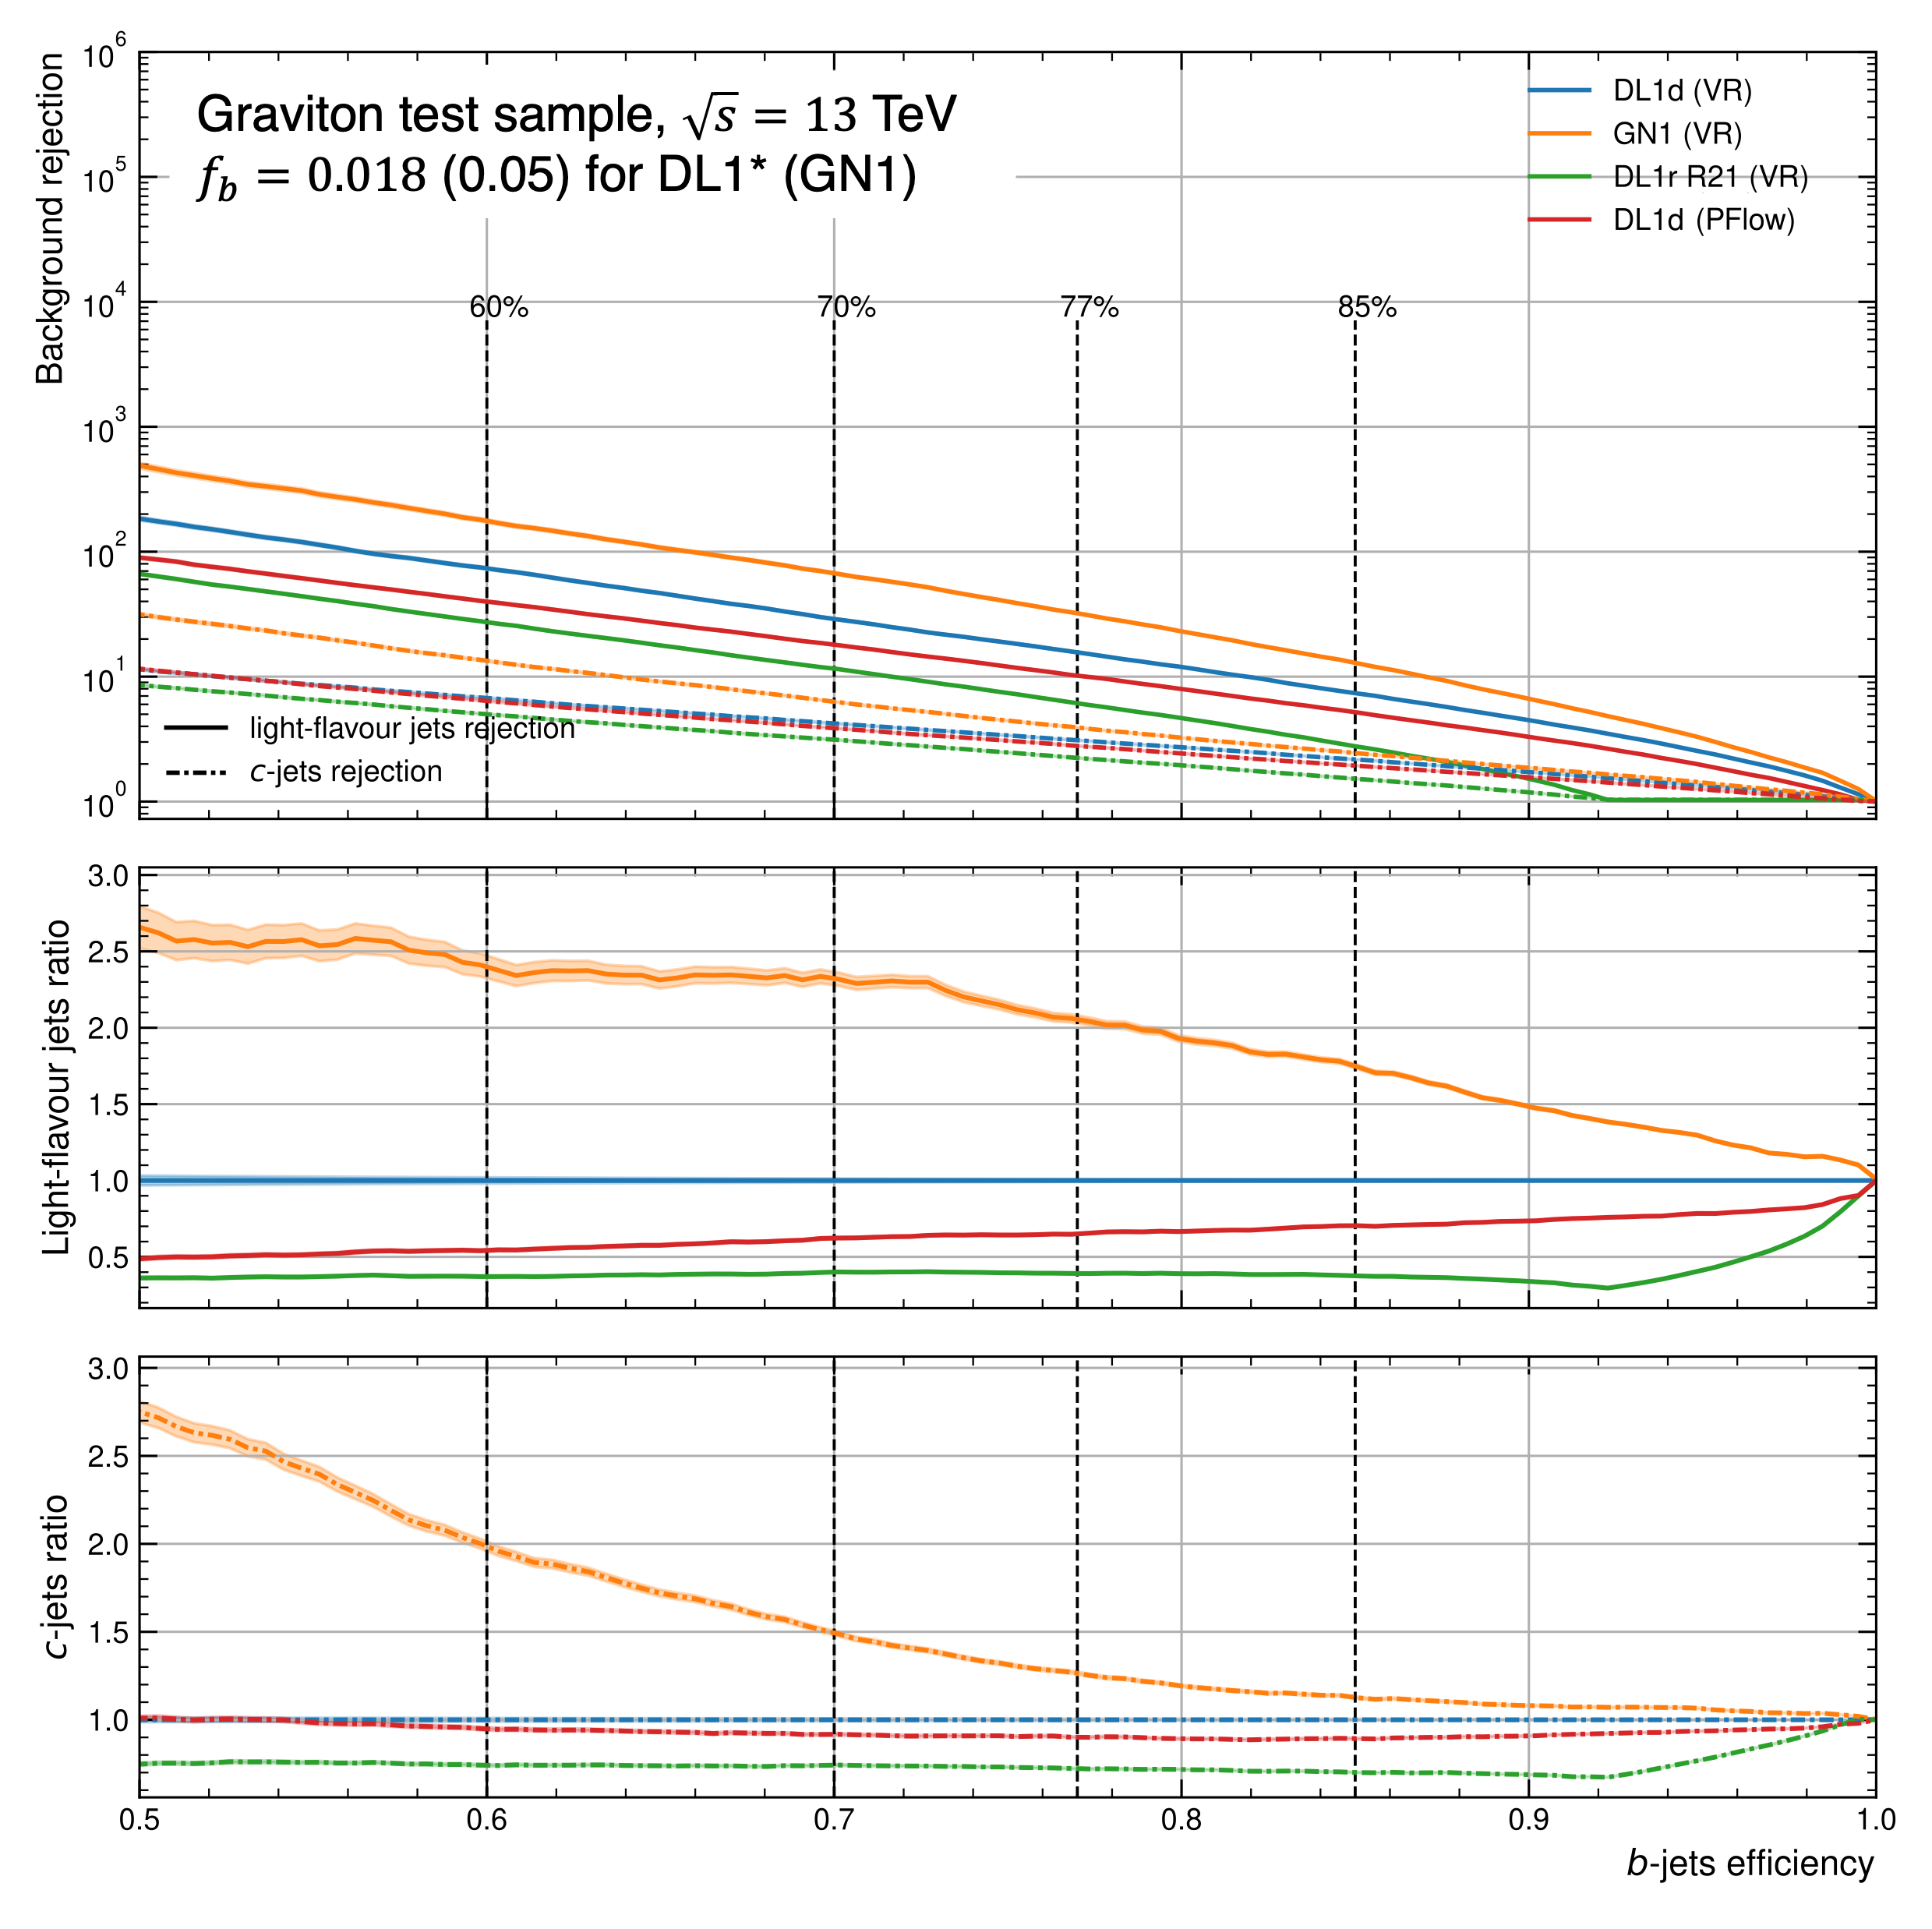
\includegraphics[width=\textwidth]{Images/FTAG/VRDL1d/ROC/grb.png}
    \caption{Graviton sample $b$-tagging, $f_c = 0.018$ for DL1d.}
    \label{fig:dl1dVRROCgr}
  \end{subfigure} \\
  \begin{subfigure}[t]{0.32\textwidth}
    \centering
    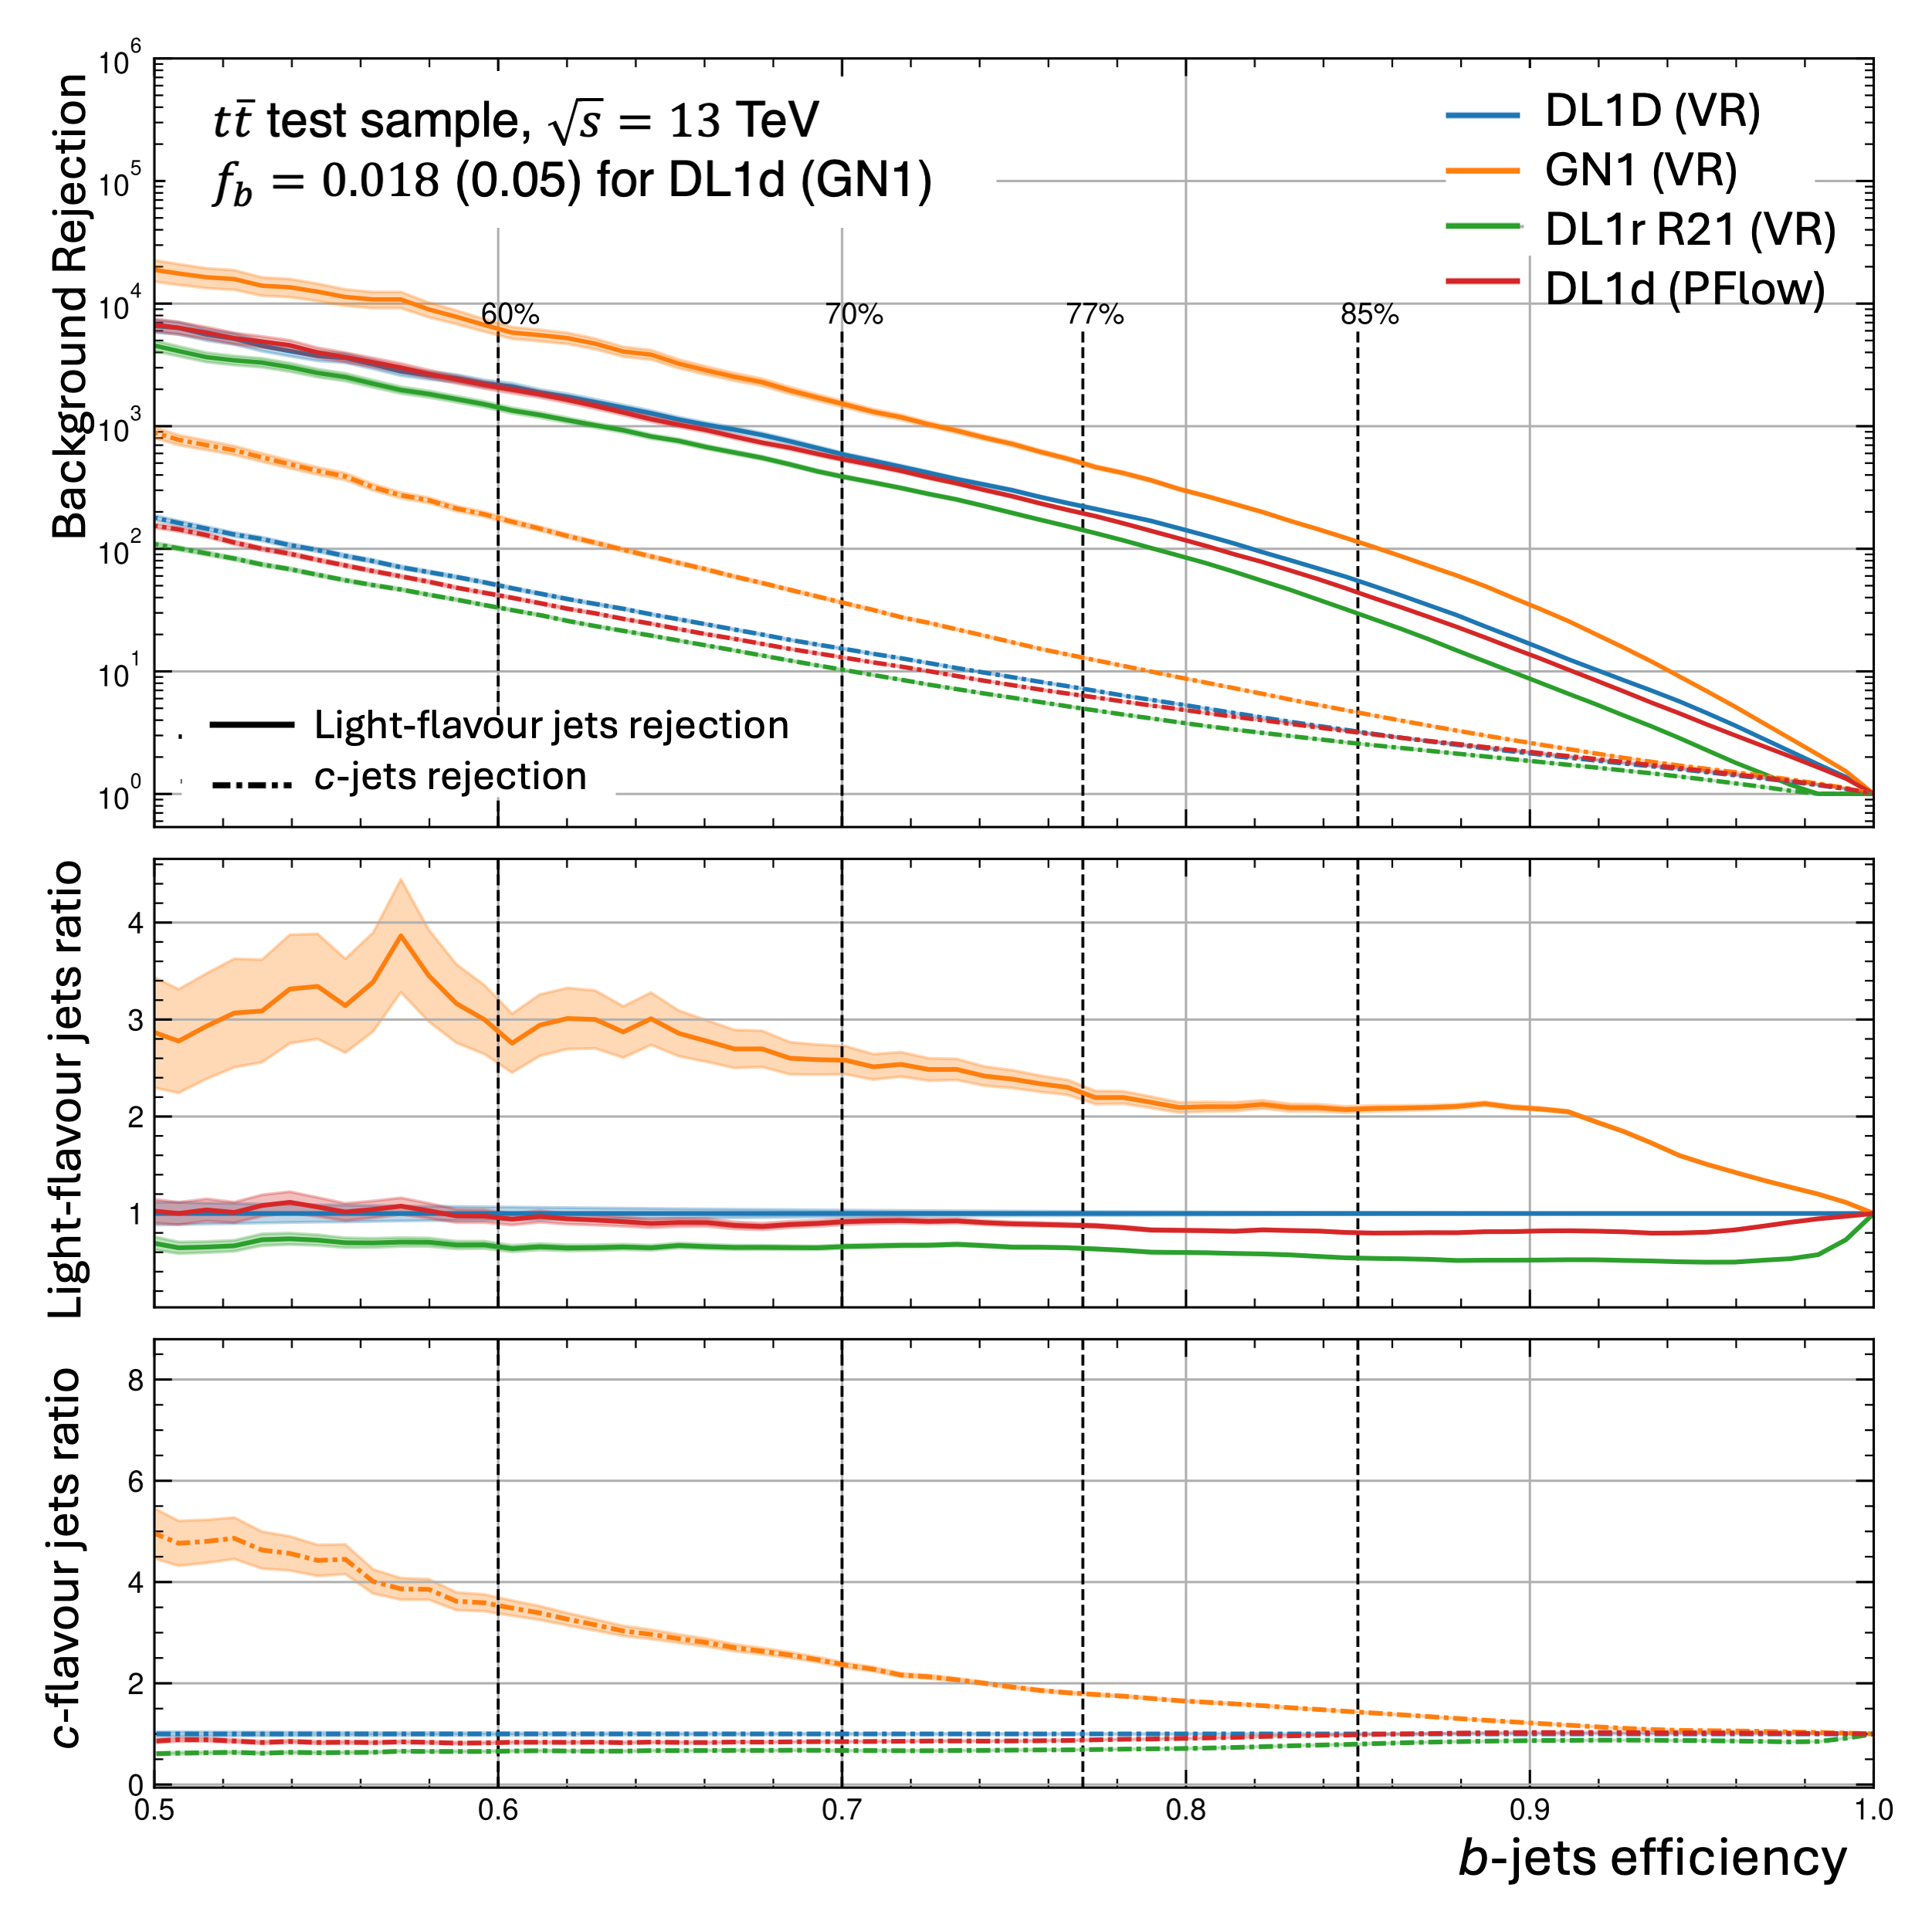
\includegraphics[width=\textwidth]{Images/FTAG/VRDL1d/ROC/ttbupf.png}
    \caption{$t\bar{t}$ test sample $b$-tagging, $f_c = 0.1$ for DL1d.}
    \label{fig:dl1dVRROCttc}
  \end{subfigure}
  \hfill
  \begin{subfigure}[t]{0.32\textwidth}
    \centering
    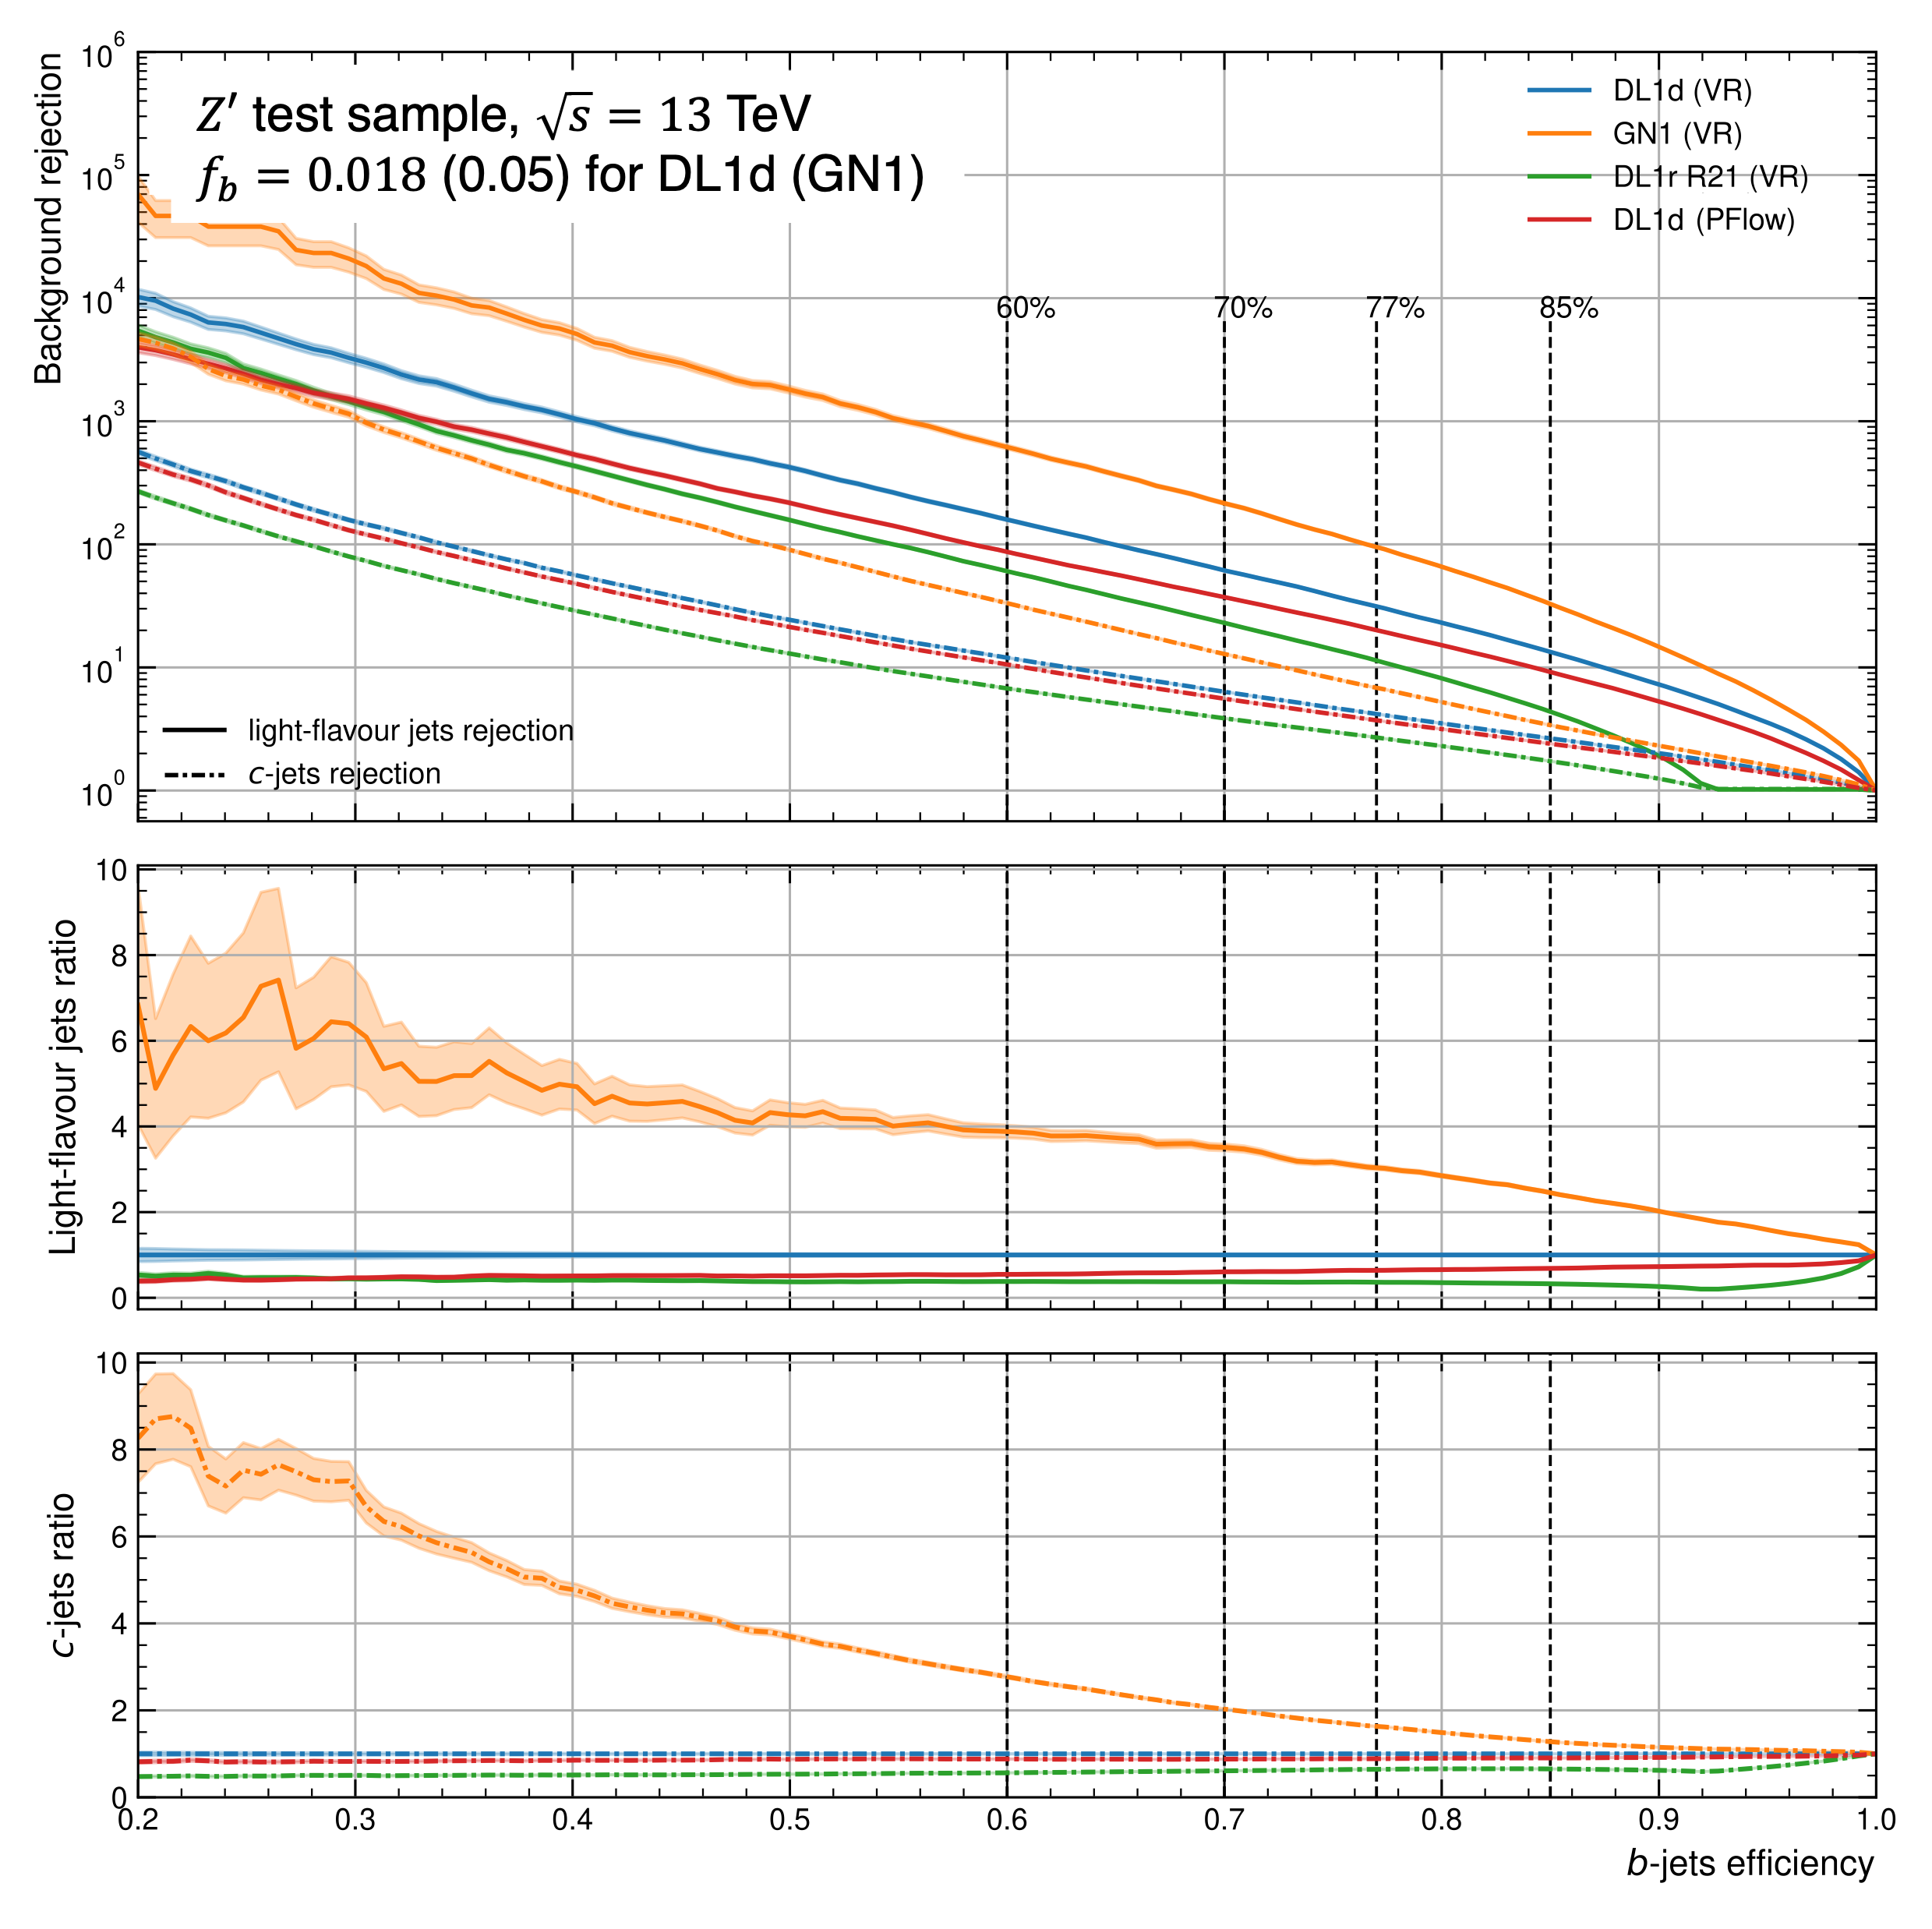
\includegraphics[width=\textwidth]{Images/FTAG/VRDL1d/ROC/zpbupf.png}
    \caption{$Z'$ test sample $b$-tagging, $f_c = 0.1$ for DL1d.}
    \label{fig:dl1dVRROCzpc}
  \end{subfigure}
  \hfill
  \begin{subfigure}[t]{0.32\textwidth}
    \centering
    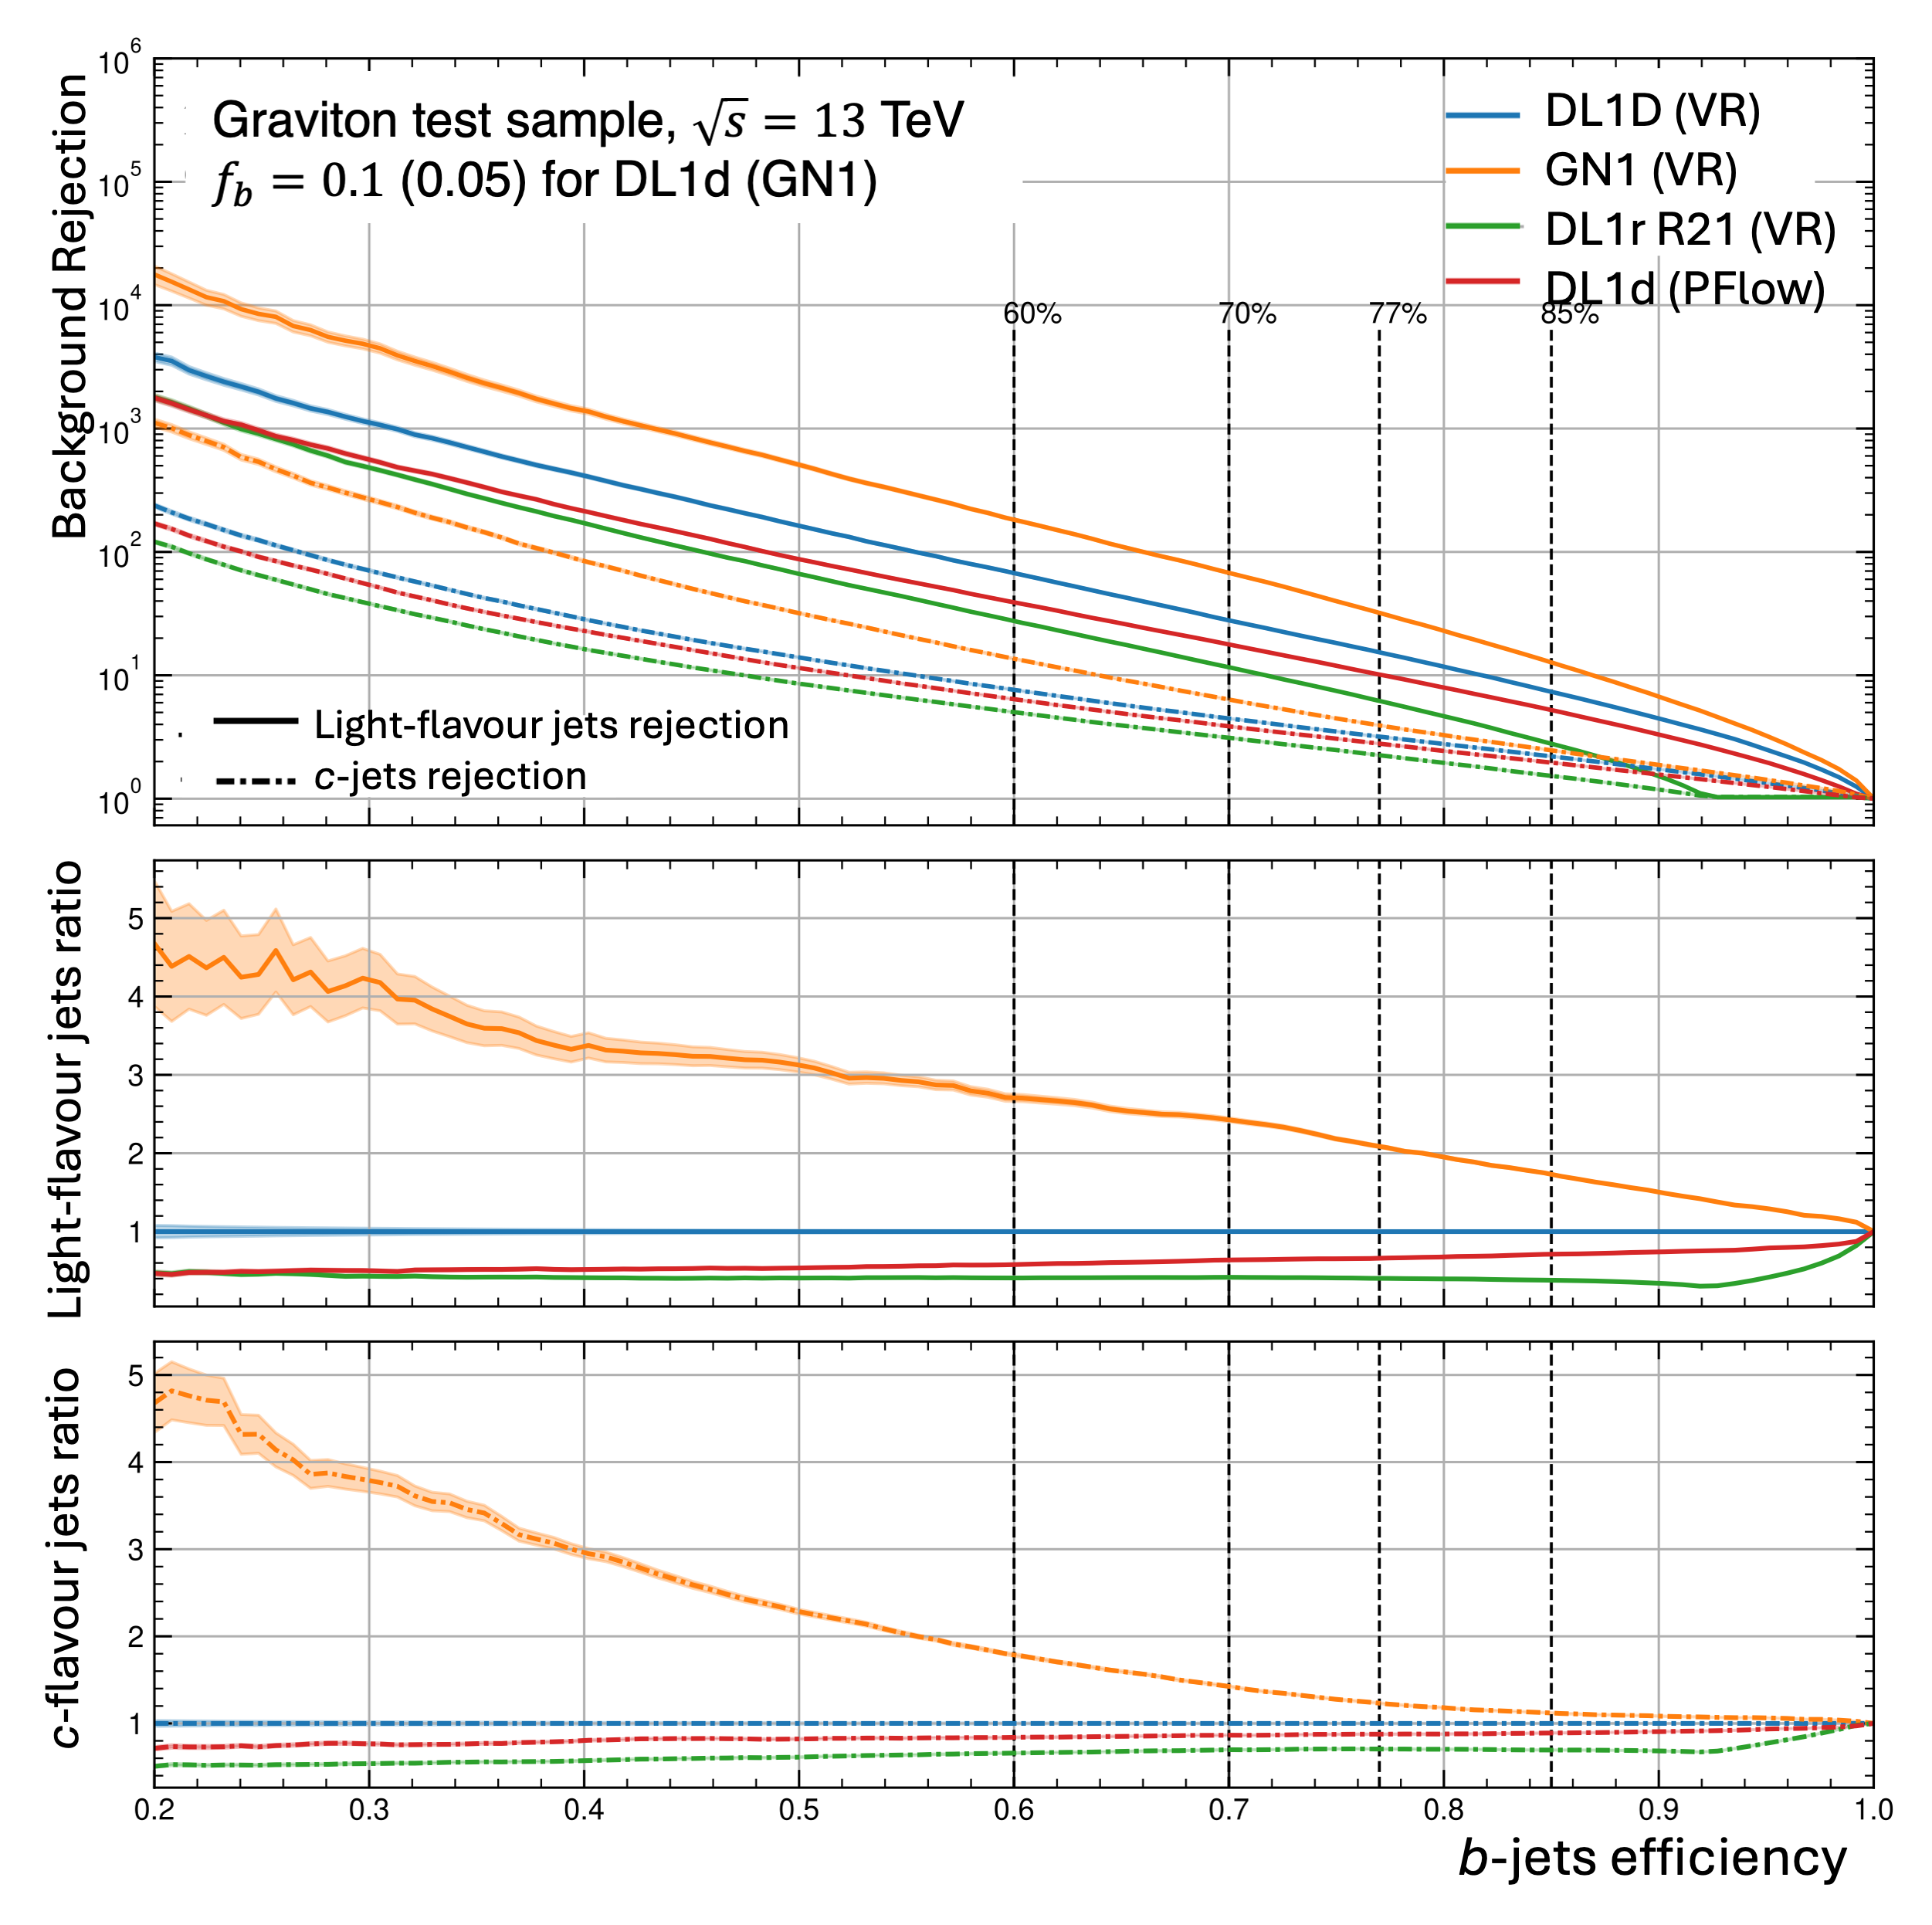
\includegraphics[width=\textwidth]{Images/FTAG/VRDL1d/ROC/grbupf.png}
    \caption{Graviton sample $b$-tagging, $f_c = 0.1$ for DL1d.}
    \label{fig:dl1dVRROCgrc}
  \end{subfigure}
  \vspace{-0.3cm}
  \caption{ROC curves for $b$-tagging. Top row uses $f_c = 0.018$ for DL1d, and bottom row $f_c = 0.1$ (GN1 $f_c = 0.05$ everywhere). The VR-jets DL1d model is in blue, a pre-release VR-trained GN1 in orange, R21 DL1r trained on VR-jets in green, and the PFlow DL1d in red.}
  \label{fig:dl1dVRROC}
\end{sidewaysfigure}